\documentclass[11pt]{article}
\usepackage[letterpaper,margin=1in]{geometry}
\usepackage[T1]{fontenc}
\usepackage{mathptmx}
\usepackage{amsmath,amssymb}
\usepackage{graphicx}
\usepackage{booktabs}
\usepackage[font=small,labelfont=bf]{caption}
\usepackage[numbers,sort&compress]{natbib}
\usepackage{xcolor}
\usepackage{microtype}
\usepackage{authblk}
\usepackage[colorlinks=true,linkcolor=blue!50!black,citecolor=blue!50!black,urlcolor=blue!50!black]{hyperref}
\setlength{\emergencystretch}{3em}
\renewcommand{\baselinestretch}{1.12}
\newcommand{\LIO}{\texorpdfstring{LaInO$_3$}{LaInO3}}
\newcommand{\BSO}{\texorpdfstring{BaSnO$_3$}{BaSnO3}}
\newcommand{\xmax}{x_\mathrm{max}}
\makeatletter\newcommand{\inputrows}[1]{\@@input #1 }\makeatother

\title{Where the gate charge must sit: electrostatic limits of electrolyte gating at the \LIO/\BSO\ interface and their intersubband signature}
\author{Gracen Ownby}
\affil{University of Oklahoma, Norman, Oklahoma, USA}
\date{\small 13 October 2026}

\begin{document}
\maketitle

\begin{abstract}
Electric-double-layer gating through a 5~nm \LIO\ cap has raised the Hall density of the \LIO/\BSO\ two-dimensional electron gas from about $5\times10^{12}$ to $1.08\times10^{14}$~cm$^{-2}$ at 150~K, falling to $7.0\times10^{13}$~cm$^{-2}$ when the same gated state is cooled to 10~K. We ask where the positive charge that balances the added electrons can sit. With a self-consistent Kane-nonparabolic Schr\"odinger--Poisson model of the interface, we place it on the cap surface, as a donor sheet inside the cap, as donors decaying from the surface, or as a uniformly doped layer next to the interface, and require that cap-localized states hold less than 1\% of the electrons. On the cap surface, as an ideal electrolyte double layer, the charge lets the cap fill by $n_s=2.8$--$3.6\times10^{13}$~cm$^{-2}$; reaching $1.08\times10^{14}$~cm$^{-2}$ that way would need a conduction-band offset of 4.7--5.1~eV, against 1.35--1.70~eV from experiment and theory, comparable to the \LIO\ gap itself. The added positive charge must instead lie, on average, within 0.42~nm of the interface at $1.08\times10^{14}$~cm$^{-2}$ and 150~K, about one \LIO\ unit cell, for clean \BSO, and within 0.17~nm for strongly compensated \BSO; at $7\times10^{13}$~cm$^{-2}$ the limits are 0.6--1.1~nm. A capacitor relation, $\xmax\approx\varepsilon_\mathrm{cap}\varepsilon_0\Delta/(e\,\delta n)$ with $\Delta$ the margin of the field-free cap, reproduces them to about 0.1~nm. As a uniformly doped layer next to the interface the charge corresponds to at least $1.3\times10^{21}$~cm$^{-3}$ of ionized donors within 0.82~nm (doubly ionized oxygen vacancies on 1.45\% of the oxygen sites), and donors decaying from the cap surface can carry at most 15\% of it. A cap permittivity of 50, twice the measured value, relaxes these distances by less than a factor of two, and over the literature ranges of the material parameters the allowed distance exceeds one unit cell in 3 of 100 parameter sets. The measured densities therefore require positive charge at the interface itself, not in an electrolyte double layer or in vacancies near the surface. Intersubband absorption cannot tell where the positive charge sits while the cap is empty, because by Gauss's law the \BSO\ side does not depend on it (mean absorption energy within 1.3\%); cap filling, in contrast, would hold the \BSO-side density near $3$--$4\times10^{13}$~cm$^{-2}$, add absorption from the cap accumulation layer and lower the mean absorption energy by 12--23\% at a given total density.
\end{abstract}

\section{Introduction}
The two-dimensional electron gas (2DEG) at the polar interface between \LIO\ and \BSO\ combines the high room-temperature mobility of \BSO\ with a polarization-induced density of a few $10^{13}$~cm$^{-2}$ \cite{Kim2019LIO,Aggoune2021}. Lee \emph{et al.} raised its density further by electric-double-layer gating with an ionic liquid on a 5~nm \LIO\ cap \cite{Lee2024LIO}. The gate voltage was applied at 220~K, above the freezing point of the liquid, and the sample was then cooled with the ions frozen. At 8~V the Hall density rose from about $5\times10^{12}$~cm$^{-2}$ without gate bias to $1.08\times10^{14}$~cm$^{-2}$ at 150~K and fell to $7.0\times10^{13}$~cm$^{-2}$ at 10~K, where the mobility reached 2100~cm$^2$/Vs, the highest reported for \BSO-based systems. The Hall resistance stayed linear up to 7~T, the sheet resistance returned almost to its initial value after some time at zero bias, and the gate leakage stayed below 2~$\mu$A at a drain current of 10~$\mu$A. Lee \emph{et al.} interpret the gating as electrostatic accumulation; they also note that ionic-liquid gating can form oxygen vacancies near the oxide surface at high bias, which can act as donors in the \LIO\ \cite{Lee2024LIO}.

Electrolyte gating can indeed act in two ways \cite{Ueno2008,Bisri2017}. In the electrostatic picture the ions form a double layer at the surface, and the gate charge sits a few \aa ngstr\"oms from it. Oxide surfaces can also be reduced: the field drives oxygen out, and the vacancies dope the material electrochemically \cite{Jeong2013,Bisri2017}. For \BSO\ films, gating has been reported to stay reversible over a wide voltage window \cite{Wang2019BSO}.

The cap decides between these pictures. If the added positive charge sits on the cap surface, the field across the cap pulls the cap conduction band down towards the surface; once it reaches the Fermi level, further electrons go into the cap instead of the \BSO\ channel. In a companion study of the intersubband (ISB) optics of this interface we found that, for an ungated density of $5\times10^{12}$~cm$^{-2}$, this happens after an added density of only $2.3$--$3.1\times10^{13}$~cm$^{-2}$ \cite{OwnbyMAT01}. Here we turn the question around and ask where the positive charge must sit for the interface to reach the measured densities with an empty cap. We map the allowed distance from the interface, the band offset an ideal double layer would need, the allowed share of donors near the surface and the minimum density of a doped layer next to the interface, for compensated and clean \BSO, three cap permittivities, two temperatures and the literature ranges of the material parameters. We then ask what ISB absorption can tell: by Gauss's law it is blind to where the positive charge sits as long as the cap is empty, but it detects cap filling.

\section{Model}
\subsection{Interface}
The model is the self-consistent interface solver of Ref.~\cite{OwnbyMAT01}, implemented in qwkit \cite{qwkit}. The conduction band of \BSO\ (band-edge mass $0.19\,m_0$, Kane nonparabolicity $\beta=0.56$~eV$^{-1}$ \cite{Niedermeier2017}, static permittivity 20) and of the \LIO\ cap (offset 1.6~eV \cite{Kim2019LIO,Lee2024LIO,Aggoune2021}, mass $0.46\,m_0$ \cite{Kim2019LIO,Aggoune2021,Jang2017LIO}, static permittivity 24 \cite{Jang2017LIO,Galazka2021}, 5~nm thick, closed by a hard wall that stands for the electrolyte) enter a one-band Schr\"odinger equation with energy-dependent mass \cite{Nelson1987}. Each subband has its own in-plane mass and nonparabolicity from the energy-dependent Hamiltonian and Fermi--Dirac occupations, and the Hartree potential follows from Poisson's equation on a 0.5~\AA\ grid. Deep acceptors in the \BSO\ deplete over a width set by Fermi-level pinning 1.0~eV below the bulk conduction band; we consider a strongly compensated layer ($N_A=5\times10^{19}$~cm$^{-3}$, the deep-acceptor density reported by Kim \emph{et al.} \cite{Kim2019LIO}) and a clean one ($10^{18}$~cm$^{-3}$), closer to the molecular-beam-epitaxy films of Ref.~\cite{Lee2024LIO}. Eight subbands enter the self-consistency; at most five are occupied, and with 14 or 20 subbands, or a 0.25~\AA\ grid, the cap fraction near the limits changes by less than $10^{-4}$. Exchange and correlation are not included. Unless stated otherwise the temperature is 300~K; the binding case, $1.08\times10^{14}$~cm$^{-2}$, is evaluated at 150~K as well.

\subsection{Placing the added positive charge}
The interface carries a fixed positive sheet $\sigma_P$ (the compensated polarization charge), chosen so that with a field-free cap the ungated density is $n_0=5\times10^{12}$~cm$^{-2}$, the value of Ref.~\cite{Lee2024LIO}. This gives $\sigma_P=4.62\times10^{13}$ and $1.01\times10^{13}$~cm$^{-2}$ for the compensated and clean layers; the difference is the depletion charge. Gating to a density $n_s$ requires the added positive charge $n_s+N_\mathrm{dep}(n_s)-\sigma_P$, which includes the small change of the depletion charge $N_\mathrm{dep}$, and we place all of it in one of the following ways:
\begin{itemize}
\item at the interface, which leaves the cap field-free (the most favourable placement);
\item as a donor sheet, 2~\AA\ wide, centred a distance $x$ inside the cap ($x\ge1$~\AA; $x=5$~nm is the cap surface);
\item on the cap surface, as an ideal electrolyte double layer;
\item as a uniformly doped layer of thickness $w$ next to the interface;
\item partly as donors decaying from the cap surface with length $\lambda=1$ or 2~nm, a model of vacancies formed at the surface, with the rest at the interface.
\end{itemize}
Donors are taken as fully ionized; the analysis constrains where the ionized (positive) charge is, whatever its origin. Because the system is neutral, the electric field on the \BSO\ side depends only on the electrons and the depletion charge, not on where in the cap the positive charge sits.

\subsection{Criterion}
We call a configuration reachable if cap-localized states (more than half of their weight in the cap) hold less than 1\% of the electrons. Once the cap starts to fill, further electrons go mostly into the cap (Sec.~\ref{sec:isb}), so the threshold marks the density beyond which the \BSO\ channel stops growing; its precise value matters little. The margin $\Delta$ between the lowest cap conduction-band energy and the Fermi level is reported as well; because the lowest cap state lies above the band edge, the 1\% criterion is reached somewhat after $\Delta$ changes sign. For each $n_s$ we find the largest sheet distance $\xmax$, the largest surface share of the donors, the largest layer thickness $w_\mathrm{max}$ and, for the double layer, the smallest offset by bisection (to 0.1~\AA, 0.002 and 0.01~eV).

\subsection{Intersubband observables}
For selected cases the self-consistent potential is extended to all subbands up to 3~eV above the ground subband, and we compute the $k=0$ time-dependent Hartree modes and the $k$-resolved random-phase response of Ref.~\cite{OwnbyMAT01}. We report the mean absorption energy $\bar E$ (the oscillator-strength-weighted mean of the $k=0$ mode energies, with the background permittivity $\varepsilon_\infty$, independent of the linewidth), the median of the absorbed power of the $k$-resolved response for a half width of 30~meV (with the polar phonons of \BSO\ in the background \cite{Stanislavchuk2012}), the ISB oscillator strength per electron $f=(2m_0/\hslash^2n_s)\sum_{a<b}(n_a-n_b)E_{ba}z_{ab}^2$, whose inverse is the optical mass, and the density held by \BSO-localized subbands, which is what a Hall measurement dominated by the high-mobility channel counts.

\section{Electrostatic limits}\label{sec:limits}
\begin{figure}[t]
\centering
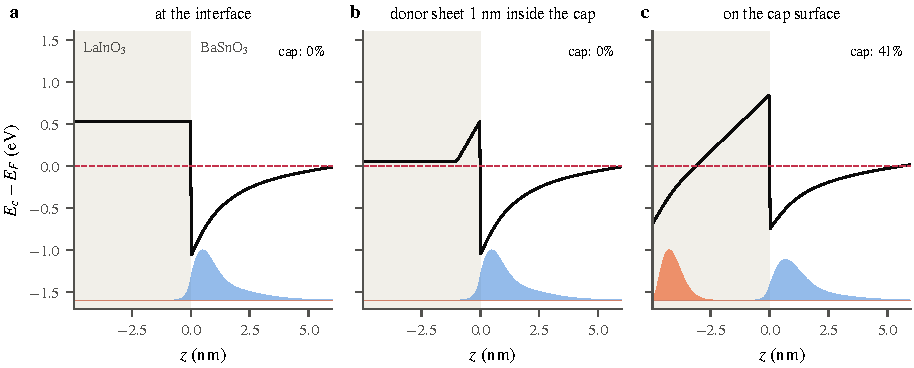
\includegraphics[width=\textwidth]{figures/fig1_profiles.pdf}
\caption{Conduction-band profile (relative to the Fermi level) and electron density in \BSO-localized (blue) and cap-localized (orange) subbands for the clean layer at $n_s=7\times10^{13}$~cm$^{-2}$ ($n_0=5\times10^{12}$~cm$^{-2}$, 300~K), with the added positive charge (a) at the interface, (b) as a donor sheet 1~nm inside the cap and (c) on the cap surface. The cap is shaded.}
\label{fig:prof}
\end{figure}

\subsection{The electrolyte double layer}
Figure~\ref{fig:prof} shows the three basic placements for the clean layer at $7\times10^{13}$~cm$^{-2}$. With the charge at the interface the cap band lies 0.53~eV above the Fermi level; with a donor sheet 1~nm inside the cap the band between the sheet and the surface is lowered to 0.05~eV above it; with the charge on the surface, the cap band falls 0.69~eV below the Fermi level at the surface, and 41\% of the electrons sit in a surface accumulation layer.

The double layer fills the cap early: cap states hold 1\% of the electrons at $n_s=2.8$ and $3.6\times10^{13}$~cm$^{-2}$ (compensated, clean) \cite{OwnbyMAT01}. Raising the offset postpones this, but slowly (Fig.~\ref{fig:lim}b): every $10^{13}$~cm$^{-2}$ of added density needs 0.42--0.46~eV more. At $7\times10^{13}$~cm$^{-2}$ the offset would have to be 3.50 (compensated) or 3.03~eV (clean), and at $1.08\times10^{14}$~cm$^{-2}$ 5.13 or 4.65~eV, against 1.35--1.70~eV from experiment and first-principles calculations \cite{Kim2019LIO,Lee2024LIO,Aggoune2021}. The gap of \LIO\ is 4.1--5.0~eV (4.35--4.39~eV for the optical gap of bulk crystals \cite{Galazka2021,Jang2017LIO,Kim2019LIO,Aggoune2021}) and that of \BSO\ about 3.0~eV \cite{Aggoune2022}; offsets above their difference, 1.1--2.0~eV, would require a staggered alignment, and those needed above $10^{14}$~cm$^{-2}$ approach or exceed the \LIO\ gap itself. A cap permittivity of 50 lowers them by 1.1--1.2~eV at $7\times10^{13}$~cm$^{-2}$ (Table~\ref{tab:map}), still far outside the measured range. The slope follows from the capacitor the cap forms: the field $e\,\delta n/\varepsilon_\mathrm{cap}\varepsilon_0$ across $d=5$~nm lowers the electron energy at the surface by $e^2\delta n\,d/\varepsilon_\mathrm{cap}\varepsilon_0=0.38$~eV per $10^{13}$~cm$^{-2}$, and the Fermi level rises at the same time.

\begin{figure}[t]
\centering
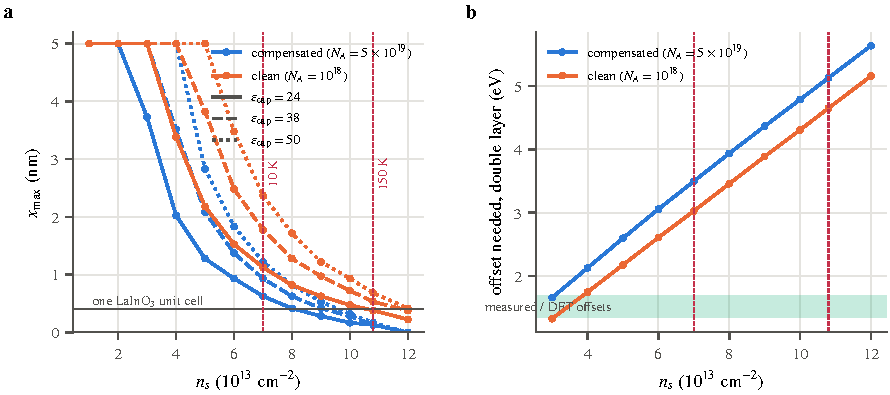
\includegraphics[width=\textwidth]{figures/fig2_limits.pdf}
\caption{(a) Largest distance $\xmax$ of the added positive charge (a donor sheet) from the interface for which cap states hold less than 1\% of the electrons, versus the gated density ($n_0=5\times10^{12}$~cm$^{-2}$, 300~K), for compensated (blue) and clean (orange) \BSO\ and cap permittivities of 24, 38 and 50. The horizontal line marks one \LIO\ pseudocubic cell (0.41~nm); the dashed lines mark the densities measured at 10 and 150~K \cite{Lee2024LIO}. (b) Conduction-band offset needed for the same criterion with all the added charge on the cap surface (cap permittivity 24); the band marks the measured and calculated offsets.}
\label{fig:lim}
\end{figure}

\subsection{How close to the interface}
Figure~\ref{fig:lim}a and Table~\ref{tab:map} give $\xmax$. Up to $3\times10^{13}$~cm$^{-2}$ the charge can sit almost anywhere in the cap. Above that, $\xmax$ falls steeply. At $7\times10^{13}$~cm$^{-2}$ it is 0.62~nm (compensated) and 1.13~nm (clean). At $1.08\times10^{14}$~cm$^{-2}$ and 150~K, the temperature at which this density was measured, it is 0.42~nm for the clean layer, about one \LIO\ unit cell, and 0.17~nm for the compensated layer, whose field-free cap is itself within 0.03~eV of filling (300~K values: 0.37 and 0.12~nm).

The limit is a capacitor relation. A sheet at distance $x$ lowers the cap band beyond it by $e^2\delta n\,x/\varepsilon_\mathrm{cap}\varepsilon_0$, so the cap stays empty while this is smaller than the margin $\Delta$ of the field-free cap:
\begin{equation}
\xmax\approx\frac{\varepsilon_\mathrm{cap}\varepsilon_0\,\Delta(n_s)}{e^2\,\delta n},\label{eq:xmax}
\end{equation}
with $\delta n$ the added charge. For a cap permittivity of 24 this reproduces the computed $\xmax$ to within 1~\AA\ from $5\times10^{13}$~cm$^{-2}$ upwards in both layers (for example 10.7 against 11.2~\AA\ for the clean layer at $7\times10^{13}$~cm$^{-2}$), and for 38 and 50 to within 1.3~\AA\ from $7\times10^{13}$~cm$^{-2}$ upwards; the estimate mostly falls slightly short because the lowest cap state lies above the band edge. Equation~\eqref{eq:xmax} makes the two ingredients explicit: the margin, which shrinks as the Fermi level rises, and the added charge, which sets the field. The cap permittivity enters only through the field: $\varepsilon_\mathrm{cap}=38$ and 50 raise $\xmax$ to 0.62 and 0.77~nm for the clean layer at $1.08\times10^{14}$~cm$^{-2}$ and 150~K.

\begin{table}[t]
\centering\small
\caption{Electrostatic limits at the measured densities ($n_0=5\times10^{12}$~cm$^{-2}$). $\xmax$: largest distance of a donor sheet carrying the added charge (values near 0.1~nm mean next to the interface); share: largest fraction of the added charge that can sit in donors decaying from the cap surface with length 1~nm (2~nm), the rest at the interface; offset: smallest conduction-band offset for an ideal double layer ($>4$: beyond the search range; the wider scan of Fig.~\ref{fig:lim}b gives 4.65--5.13~eV for permittivity 24 at 300~K).}
\label{tab:map}
\begin{tabular}{@{}llcccccc@{}}
\toprule
& & \multicolumn{3}{c}{$n_s=7.0\times10^{13}$~cm$^{-2}$} & \multicolumn{3}{c}{$n_s=1.08\times10^{14}$~cm$^{-2}$} \\
\cmidrule(lr){3-5}\cmidrule(lr){6-8}
\BSO, $T$ & $\varepsilon_\mathrm{cap}$ & $\xmax$ (nm) & share & offset (eV) & $\xmax$ (nm) & share & offset (eV) \\ \midrule
\inputrows{table_map.tex}
\bottomrule
\end{tabular}
\end{table}

\subsection{Distributed donors}
Donors formed at the cap surface and decaying into it are nearly as harmful as the double layer. With a decay length of 1--2~nm and the rest of the added charge at the interface, at most 21--24\% (compensated) or 36--40\% (clean) of it can sit in such donors at $7\times10^{13}$~cm$^{-2}$, and at most 5--6\% or 13--15\% at $1.08\times10^{14}$~cm$^{-2}$ and 150~K (Table~\ref{tab:map}).

A uniformly doped layer next to the interface is the natural form of the charge if donors accumulate there. At $7\times10^{13}$~cm$^{-2}$ its thickness must stay below $w_\mathrm{max}=1.22$~nm (compensated) or 2.27~nm (clean), so that its ionized-donor density must exceed $5.7\times10^{20}$ or $2.9\times10^{20}$~cm$^{-3}$. At $1.08\times10^{14}$~cm$^{-2}$ and 150~K the clean layer needs $w\le0.82$~nm and at least $1.3\times10^{21}$~cm$^{-3}$; as doubly ionized oxygen vacancies ($6.3\times10^{20}$~cm$^{-3}$) this is 1.45\% of the oxygen sites of \LIO\ (three per pseudocubic cell of 4.1~\AA), in its first two unit cells. The compensated layer needs $w\le0.32$~nm and $3.4\times10^{21}$~cm$^{-3}$ (3.9\% of the sites). This assumes that the donors are ionized, i.e. that their levels lie above the Fermi level, which near the interface is only the margin $\Delta$, 0.03--0.23~eV, below the \LIO\ conduction band; deeper donors would be neutral there and could not supply the charge.

\subsection{Temperature, permittivity and material parameters}\label{sec:uq}
Lowering the temperature from 300 to 150~K raises $\xmax$ by at most 0.16~nm and lowers the offsets by at most 0.04~eV at the measured densities (Table~\ref{tab:map}). The cap permittivity matters more, through Eq.~\eqref{eq:xmax}: a value of 50, twice the measured one, raises the limits by factors of 1.4--2.1, to 0.28--0.77~nm at $1.08\times10^{14}$~cm$^{-2}$ and 150~K.

\begin{figure}[t]
\centering
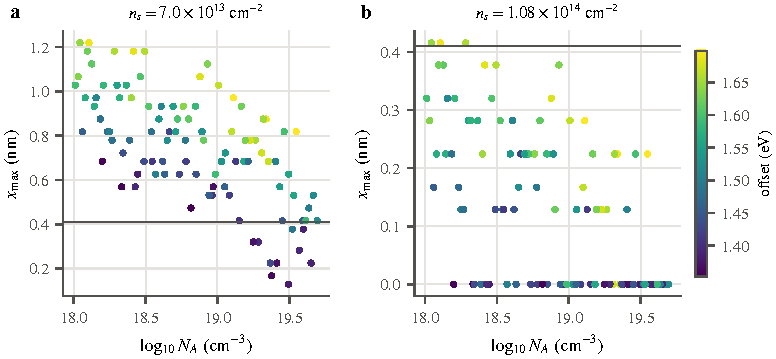
\includegraphics[width=0.85\textwidth]{figures/fig4_uq.pdf}
\caption{Largest distance $\xmax$ of the added positive charge from the interface for the 100 parameter sets of the uncertainty analysis, at the two measured densities ($n_0=5\times10^{12}$~cm$^{-2}$, cap permittivity 24, 300~K), against the acceptor density and colored by the conduction-band offset. $\xmax=0$: cap states hold more than 1\% of the electrons even with the donor sheet next to the interface. The horizontal line marks one \LIO\ unit cell.}
\label{fig:uq}
\end{figure}

The material parameters are uncertain as well. We repeated the search for $\xmax$ over the 100 Latin-hypercube parameter sets of the uncertainty analysis of Ref.~\cite{OwnbyMAT01} (300~K): \BSO\ band-edge mass 0.17--0.22~$m_0$, nonparabolicity 0.25--0.56~eV$^{-1}$ \cite{Niedermeier2017,Krishnaswamy2017}, $\varepsilon_\infty=3.3$--4.3 (with the static permittivity from the Lyddane--Sachs--Teller relation), offset 1.35--1.70~eV, cap mass 0.30--0.50~$m_0$, acceptor density $10^{18}$--$5\times10^{19}$~cm$^{-3}$ (log-uniform) and pinning 0.5--1.5~eV. At $7\times10^{13}$~cm$^{-2}$ the 5th, 50th and 95th percentiles of $\xmax$ are 0.28, 0.78 and 1.18~nm, and in no parameter set may the charge sit even halfway across the cap (Fig.~\ref{fig:uq}a). At $1.08\times10^{14}$~cm$^{-2}$ the field-free cap itself fills in 22 of the 100 sets, the median of $\xmax$ is 0.13~nm and the 95th percentile 0.38~nm, and $\xmax$ exceeds one unit cell in 3 sets (at most 0.42~nm; Fig.~\ref{fig:uq}b). The rank correlations single out the offset ($+0.73$ and $+0.67$ at the two densities) and the acceptor density ($-0.66$, $-0.55$), followed by $\varepsilon_\infty$ and the mass ($+0.19$ to $+0.30$): a larger offset and less compensation both widen the margin $\Delta$ of Eq.~\eqref{eq:xmax}.

\section{What the intersubband response sees}\label{sec:isb}
\begin{figure}[t]
\centering
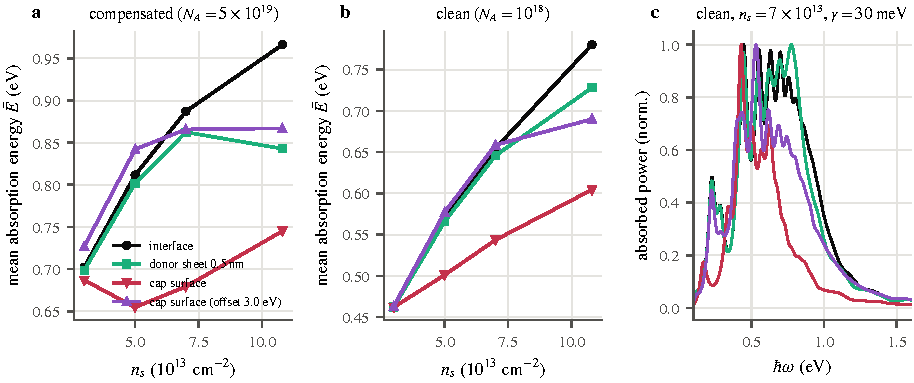
\includegraphics[width=\textwidth]{figures/fig3_isb.pdf}
\caption{(a, b) Mean absorption energy $\bar E$ of the collective ISB response versus the gated density for four placements of the added positive charge: at the interface, as a donor sheet 0.5~nm inside the cap, on the cap surface, and on the cap surface with a 3.0~eV offset (300~K). (c) Absorbed power (half width 30~meV, normalized to its maximum) for the clean layer at $7\times10^{13}$~cm$^{-2}$.}
\label{fig:isb}
\end{figure}

Gauss's law fixes the field on the \BSO\ side by the electrons and the depletion charge alone. As long as the cap is empty, where the positive charge sits in the cap changes only the tails of the subbands in the cap. With a donor sheet 0.5~nm inside the cap instead of at the interface, and a margin of at least 0.29~eV, $E_{21}$ changes by at most 3~meV, the mean absorption energy by at most 1.3\% and the median of the absorption by at most 1.4\% (Fig.~\ref{fig:isb}). Close to the limit the response becomes sensitive to the cap states that approach the Fermi level: for the compensated layer at $7\times10^{13}$~cm$^{-2}$, with a margin of 0.06~eV and 0.2\% of the electrons in the cap, $\bar E$ is 2.8\% and the median 9\% lower. A larger offset (3.0~eV, with the charge on the surface and the cap empty) changes $\bar E$ by up to 3.8\%, through the upper subbands that reach into the cap, but leaves the median within 1.9\%. The ISB response therefore cannot distinguish charge at the interface from donors close to it or from a larger offset.

It does register cap filling. With the charge on the cap surface, cap states take up the added electrons: from $5\times10^{13}$~cm$^{-2}$ upwards the density in \BSO-localized subbands stays at $3.2$--$3.6\times10^{13}$~cm$^{-2}$ (compensated) and $3.9$--$4.4\times10^{13}$~cm$^{-2}$ (clean). At a given total density the mean absorption energy is then 12--23\% lower than with the charge at the interface (0.66--0.75 against 0.81--0.97~eV, compensated; 0.50--0.60 against 0.57--0.78~eV, clean), the absorption gains lines from the cap accumulation layer (Fig.~\ref{fig:isb}c), and the ISB oscillator strength per electron falls from 3.1--3.4 to 2.4--2.9 (compensated) and from 3.5--3.9 to 2.9--3.5 (clean), because the cap electrons are heavier. Compared at the same \BSO-side density, the quantity a Hall measurement would count, the mean absorption energy differs from that of the field-free case by $-8$\% to $+13$\%, so $\bar E$ alone is not a clean indicator; the stalled \BSO-side density and the additional low-energy absorption are. With the charge at the interface the oscillator strength per electron corresponds to an optical mass of 0.25--0.29~$m_0$ (clean) and 0.29--0.32~$m_0$ (compensated), rising with density through the nonparabolicity.

For the measured gating this means that a Hall density of $1.08\times10^{14}$~cm$^{-2}$ is itself incompatible with a filled cap in this model, since cap filling would hold the \BSO-side density below $4.4\times10^{13}$~cm$^{-2}$. ISB absorption on such a sample would follow the field-free curve of Fig.~\ref{fig:isb}a,b at the \BSO-side density, whatever the gating mechanism, and would thus measure that density optically and independently of the mobility.

\section{Discussion}\label{sec:disc}
\emph{What the measured densities imply.} The Hall density of Ref.~\cite{Lee2024LIO} counts the high-mobility carriers. A low-mobility channel near the cap surface would add little to it, and a sizeable parallel channel would bend the Hall resistance, since $\mu B\approx1.5$ at 7~T for the 2DEG at 10~K; the Hall resistance stayed linear. A Hall density of $1.08\times10^{14}$~cm$^{-2}$ therefore means that many electrons in the \BSO\ channel, and in this model that requires the balancing positive charge within about one \LIO\ unit cell of the interface for clean \BSO\ and within a fraction of a cell for compensated \BSO. That is not the double layer of an electrostatic gate, which sits 5~nm away, and it is not the vacancies near the oxide surface that Lee \emph{et al.} mention, which can carry at most 15\% of the charge. The measured density points instead to chemistry at the interface: donors created in the first \LIO\ unit cell, or a change of the interface itself (more polarization charge, or donors on the \BSO\ side). For vacancies formed at the surface to end up there, oxygen or vacancies would have to migrate through the 5~nm cap during gating at 220~K; whether that is possible we cannot judge. The slow recovery of the sheet resistance at zero bias is consistent with a reversible electrochemical process.

\emph{The drop on cooling.} With the ions frozen, the positive charge is the same at 150 and 10~K, yet the Hall density falls from $1.08\times10^{14}$ to $7.0\times10^{13}$~cm$^{-2}$. Electrons do not disappear at fixed positive charge, so either the Hall density undercounts them, which happens when the occupied subbands differ in mobility, or about $3.8\times10^{13}$~cm$^{-2}$ of them stop conducting. The electrostatic limits found here change by less than 0.16~nm between 300 and 150~K and do not decide between these. A companion transport analysis \cite{OwnbyMAT03} finds that, at 7~V, the published magnetoresistance, flat between 2 and 7~T, requires about a quarter of the electrons to be nearly immobile, which the identified scattering does not produce; these electrons are not captured on cooling by traps with levels fixed relative to the band, which at fixed total charge would lower the Fermi level by 0.1--0.3~eV; how they become immobile remains open.

\emph{Alternatives within the model.} Three parameters could relax the limits. A larger offset helps little: every 0.1~eV raises the margin $\Delta$ by about as much and, by Eq.~\eqref{eq:xmax}, $\xmax$ by only 1.4~\AA\ at $10^{14}$~cm$^{-2}$. A larger cap permittivity helps in proportion, but the measured values are 23.7--24.6 \cite{Jang2017LIO,Galazka2021}. Less compensation of the \BSO\ widens the margin; together with the offset it dominates the uncertainty analysis (Sec.~\ref{sec:uq}), but within the literature ranges the allowed distance at $1.08\times10^{14}$~cm$^{-2}$ exceeds one unit cell in only 3 of 100 parameter sets.

\emph{Limitations.} The envelope-function model is at its limit for confinement within one or two unit cells \cite{OwnbyMAT01}, and the 0.1--0.4~nm distances found at $1.08\times10^{14}$~cm$^{-2}$ are below the scale on which it describes the interface; they should be read as ``at the interface''. The cap is a continuum with a hard wall and a linear permittivity; the ungated cap is assumed field-free, which in the interface-polarization picture of Ref.~\cite{Kim2019LIO} need not hold. The donors are smeared over a 2~\AA\ sheet or a uniform layer and taken as ionized. Exchange and correlation are not included; in the local approximation, screened by the static permittivity, they widen the margin by 0.04--0.05~eV \cite{OwnbyMAT01}, which by Eq.~\eqref{eq:xmax} adds less than 1~\AA\ to $\xmax$ at $10^{14}$~cm$^{-2}$ (screened by $\varepsilon_\infty$, an upper limit, they widen it by up to 0.29~eV, or about 4~\AA). The Hall density is taken as the \BSO-side density.

\section{Conclusion}
For the \LIO/\BSO\ 2DEG gated through a 5~nm \LIO\ cap, the positive charge that balances the measured electron densities cannot sit in an electrolyte double layer: the cap fills by $2.8$--$3.6\times10^{13}$~cm$^{-2}$, and offsets of 4.7--5.1~eV would be needed instead of 1.35--1.70~eV. At $1.08\times10^{14}$~cm$^{-2}$ the charge must lie within about one unit cell of the interface for clean \BSO\ and within a fraction of a cell for compensated \BSO; as a doped layer next to the interface this means $10^{21}$~cm$^{-3}$ of ionized donors, oxygen vacancies on 1.5--4\% of the sites, while donors near the cap surface can carry at most 15\% of it. A capacitor relation captures these limits. The measured densities therefore require positive charge at the interface itself. Intersubband absorption is insensitive to where the positive charge sits while the cap is empty, which makes it an optical measure of the \BSO-side density whatever the gating mechanism, and it registers cap filling through a stalled density and additional absorption from the cap. The calculations use qwkit \cite{qwkit}.

\bibliographystyle{unsrtnat}
\bibliography{refs}
\end{document}
